\chapter{Design}

\begin{longtabu} to \linewidth{@{}l l l X[j]@{}}
    Version &    Dato &    Ansvarlig &    Beskrivelse\\[-1ex]
    \midrule
    
\label{version_Systemark}
\end{longtabu}

\section{Indledning}

  
\section{Hardware arkitektur}
I følgende afsnit beskrives hvordan blodtryksmåler systemet og nogle af dets delkomponenter er opbygget.
\\
\begin{figure}[H]
	\centering
	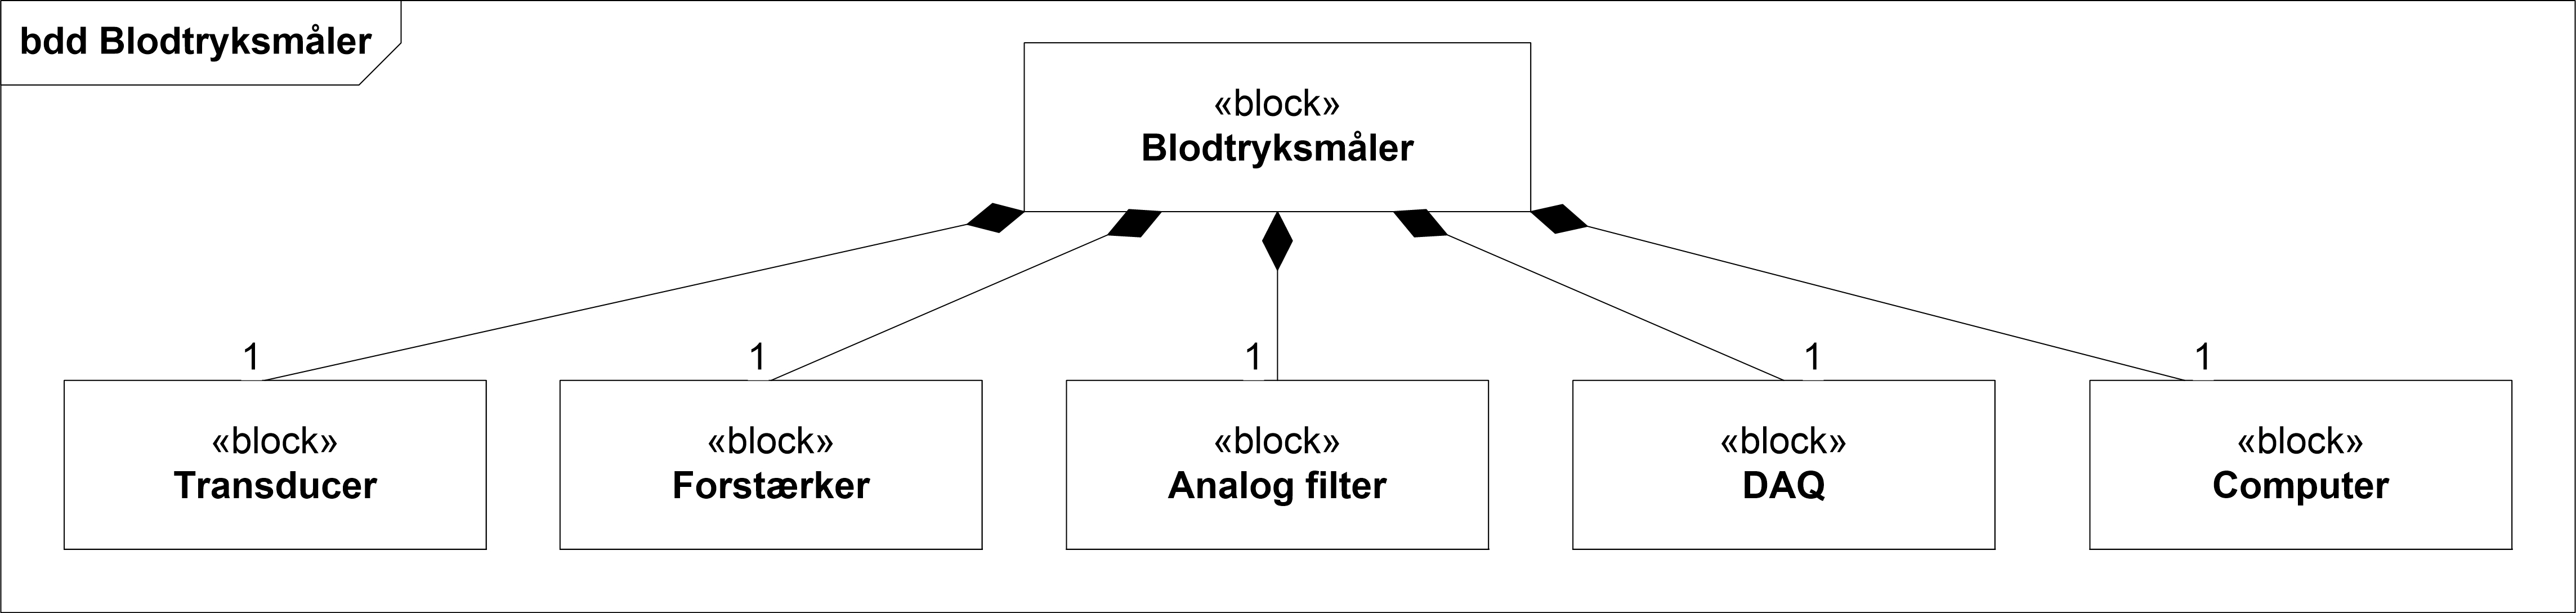
\includegraphics[width=1\textwidth]{Figurer/Hardware/BDD1}
	\caption{Blokdiagram for blodtryksmåler systemet.}
	\label{BDD blodtryksmaaler}
\end{figure}

Ud af blokdiagrammet, figur \ref{BDD blodtryksmaaler}, kan man se at blodtryksmåler systemet består af en transducer, en forstærker, et analogt filter, en DAQ og en computer.\\
\begin{figure}[H]
	\centering
	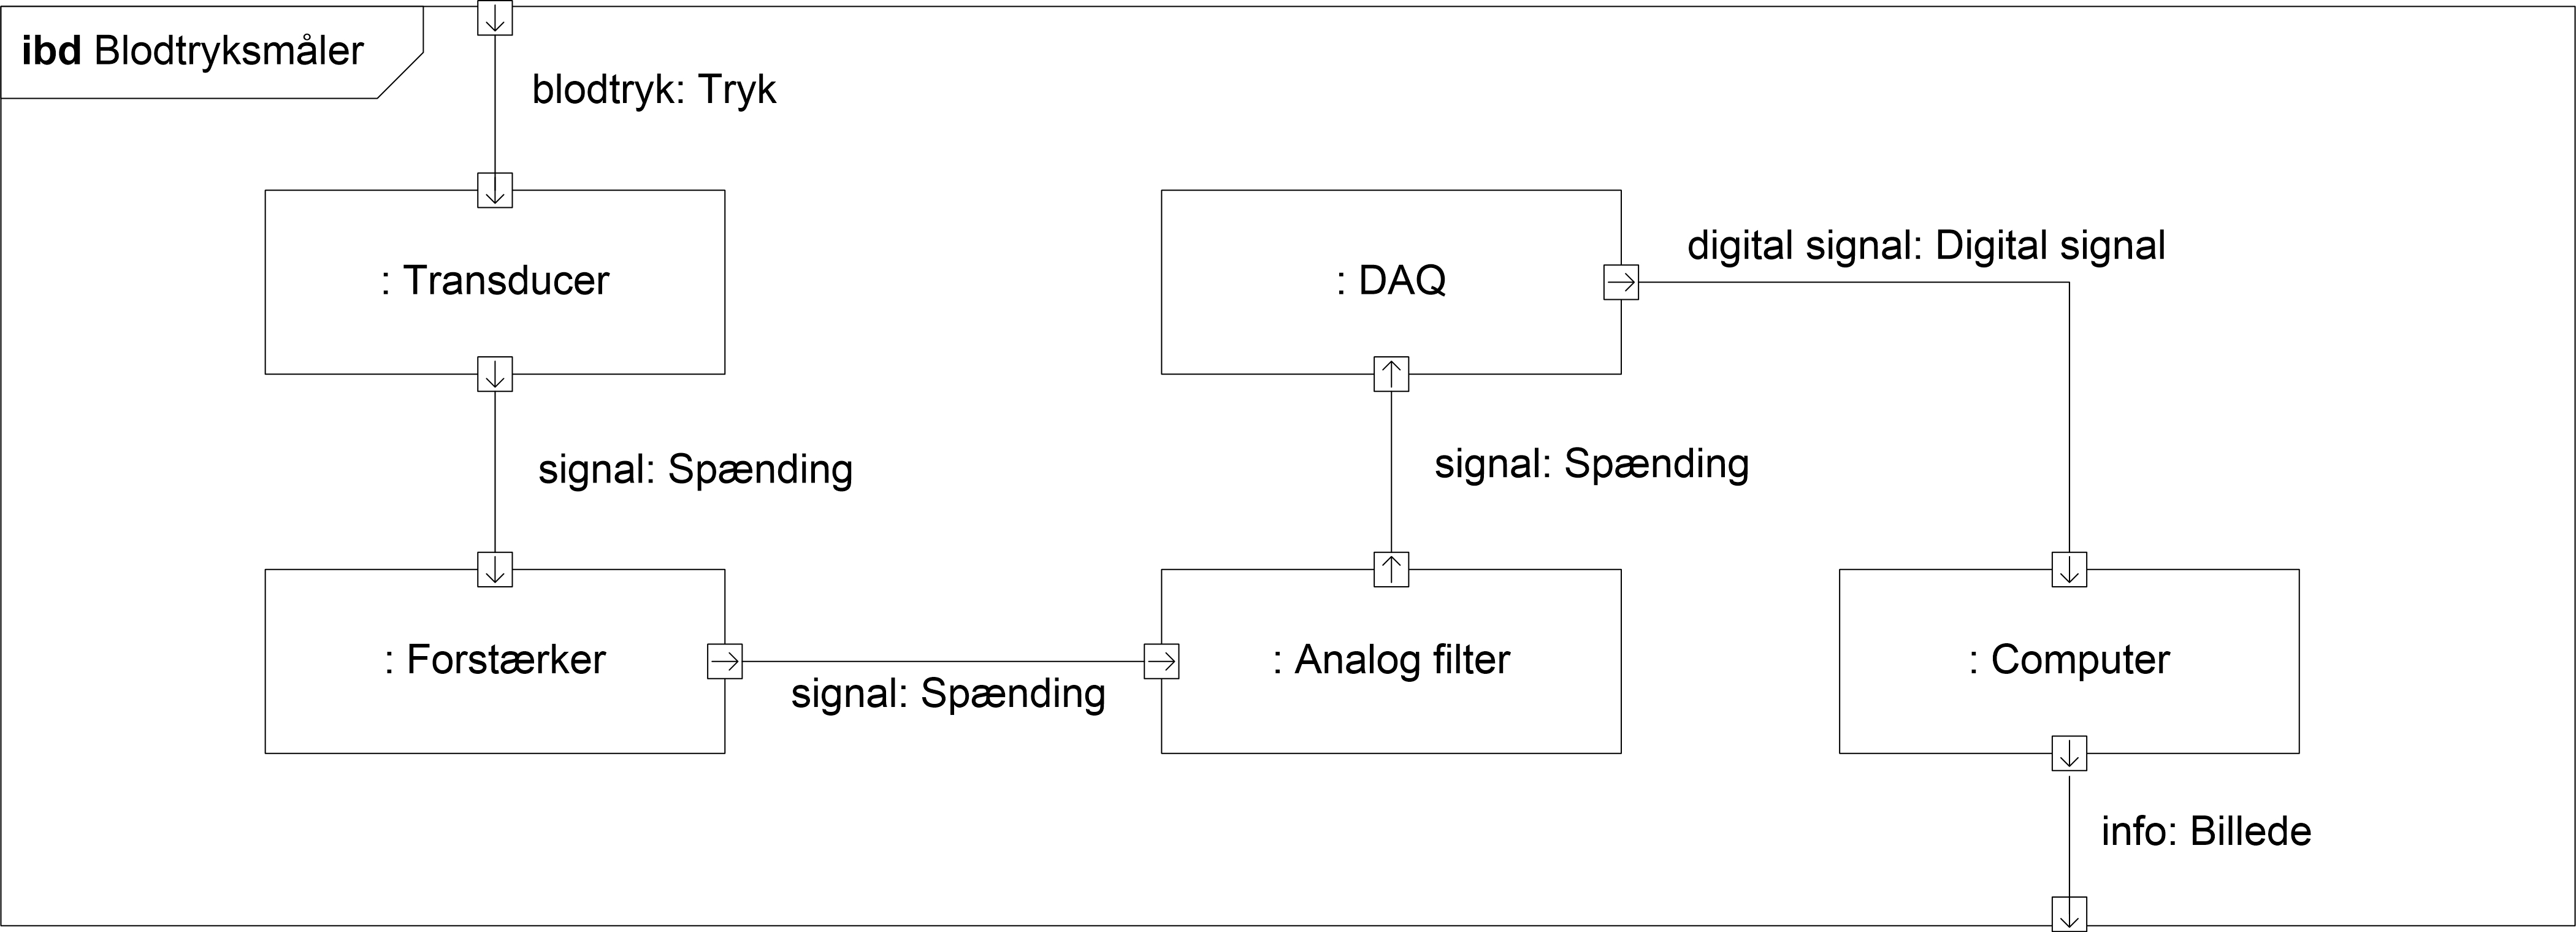
\includegraphics[width=1\textwidth]{Figurer/Hardware/IBD}
	\caption{Internt blok diagram for blodtryksmåler systemet.}
	\label{IBD blodtryksmaaler}
\end{figure}

Ud af det interne blok diagram, figur \ref{IBD blodtryksmaaler}, kan ses det at blodtrykket i form af det målte tryk kommer ind i transduceren. Transduceren som omformer det målte tryk til et spændingssignal, sender signalet vidre til forstærkeren. Fra forstærkeren sendes signalet over i det analoge filter og derfra ind i DAQ'en. Endeligt sendes det digitale signal fra DAQ'en over i en computer, der fortolker signalet som et billede, der vises til omverdenen.

\subsection{Design af forstærker}
Forstærkeren er designet med tanke på, at det er meget små spændinger der arbejdes med. Grundet dette, er en almindelig operationsforstærker fravalgt, da dens reelle indgangsimpedans er for lille. En Instrumentationsforstærkers indgangsimpedans i den virkelige verden, er højere, og den kan dermed opfange meget små signaler så som blodtryk.\\
Vejleder rådede herefter til at projektgruppen brugte instrumentationsforstærkeren INA114. Forstærkerens design kan ses på figur X.\\ 
\begin{figure}[H]
	\centering
	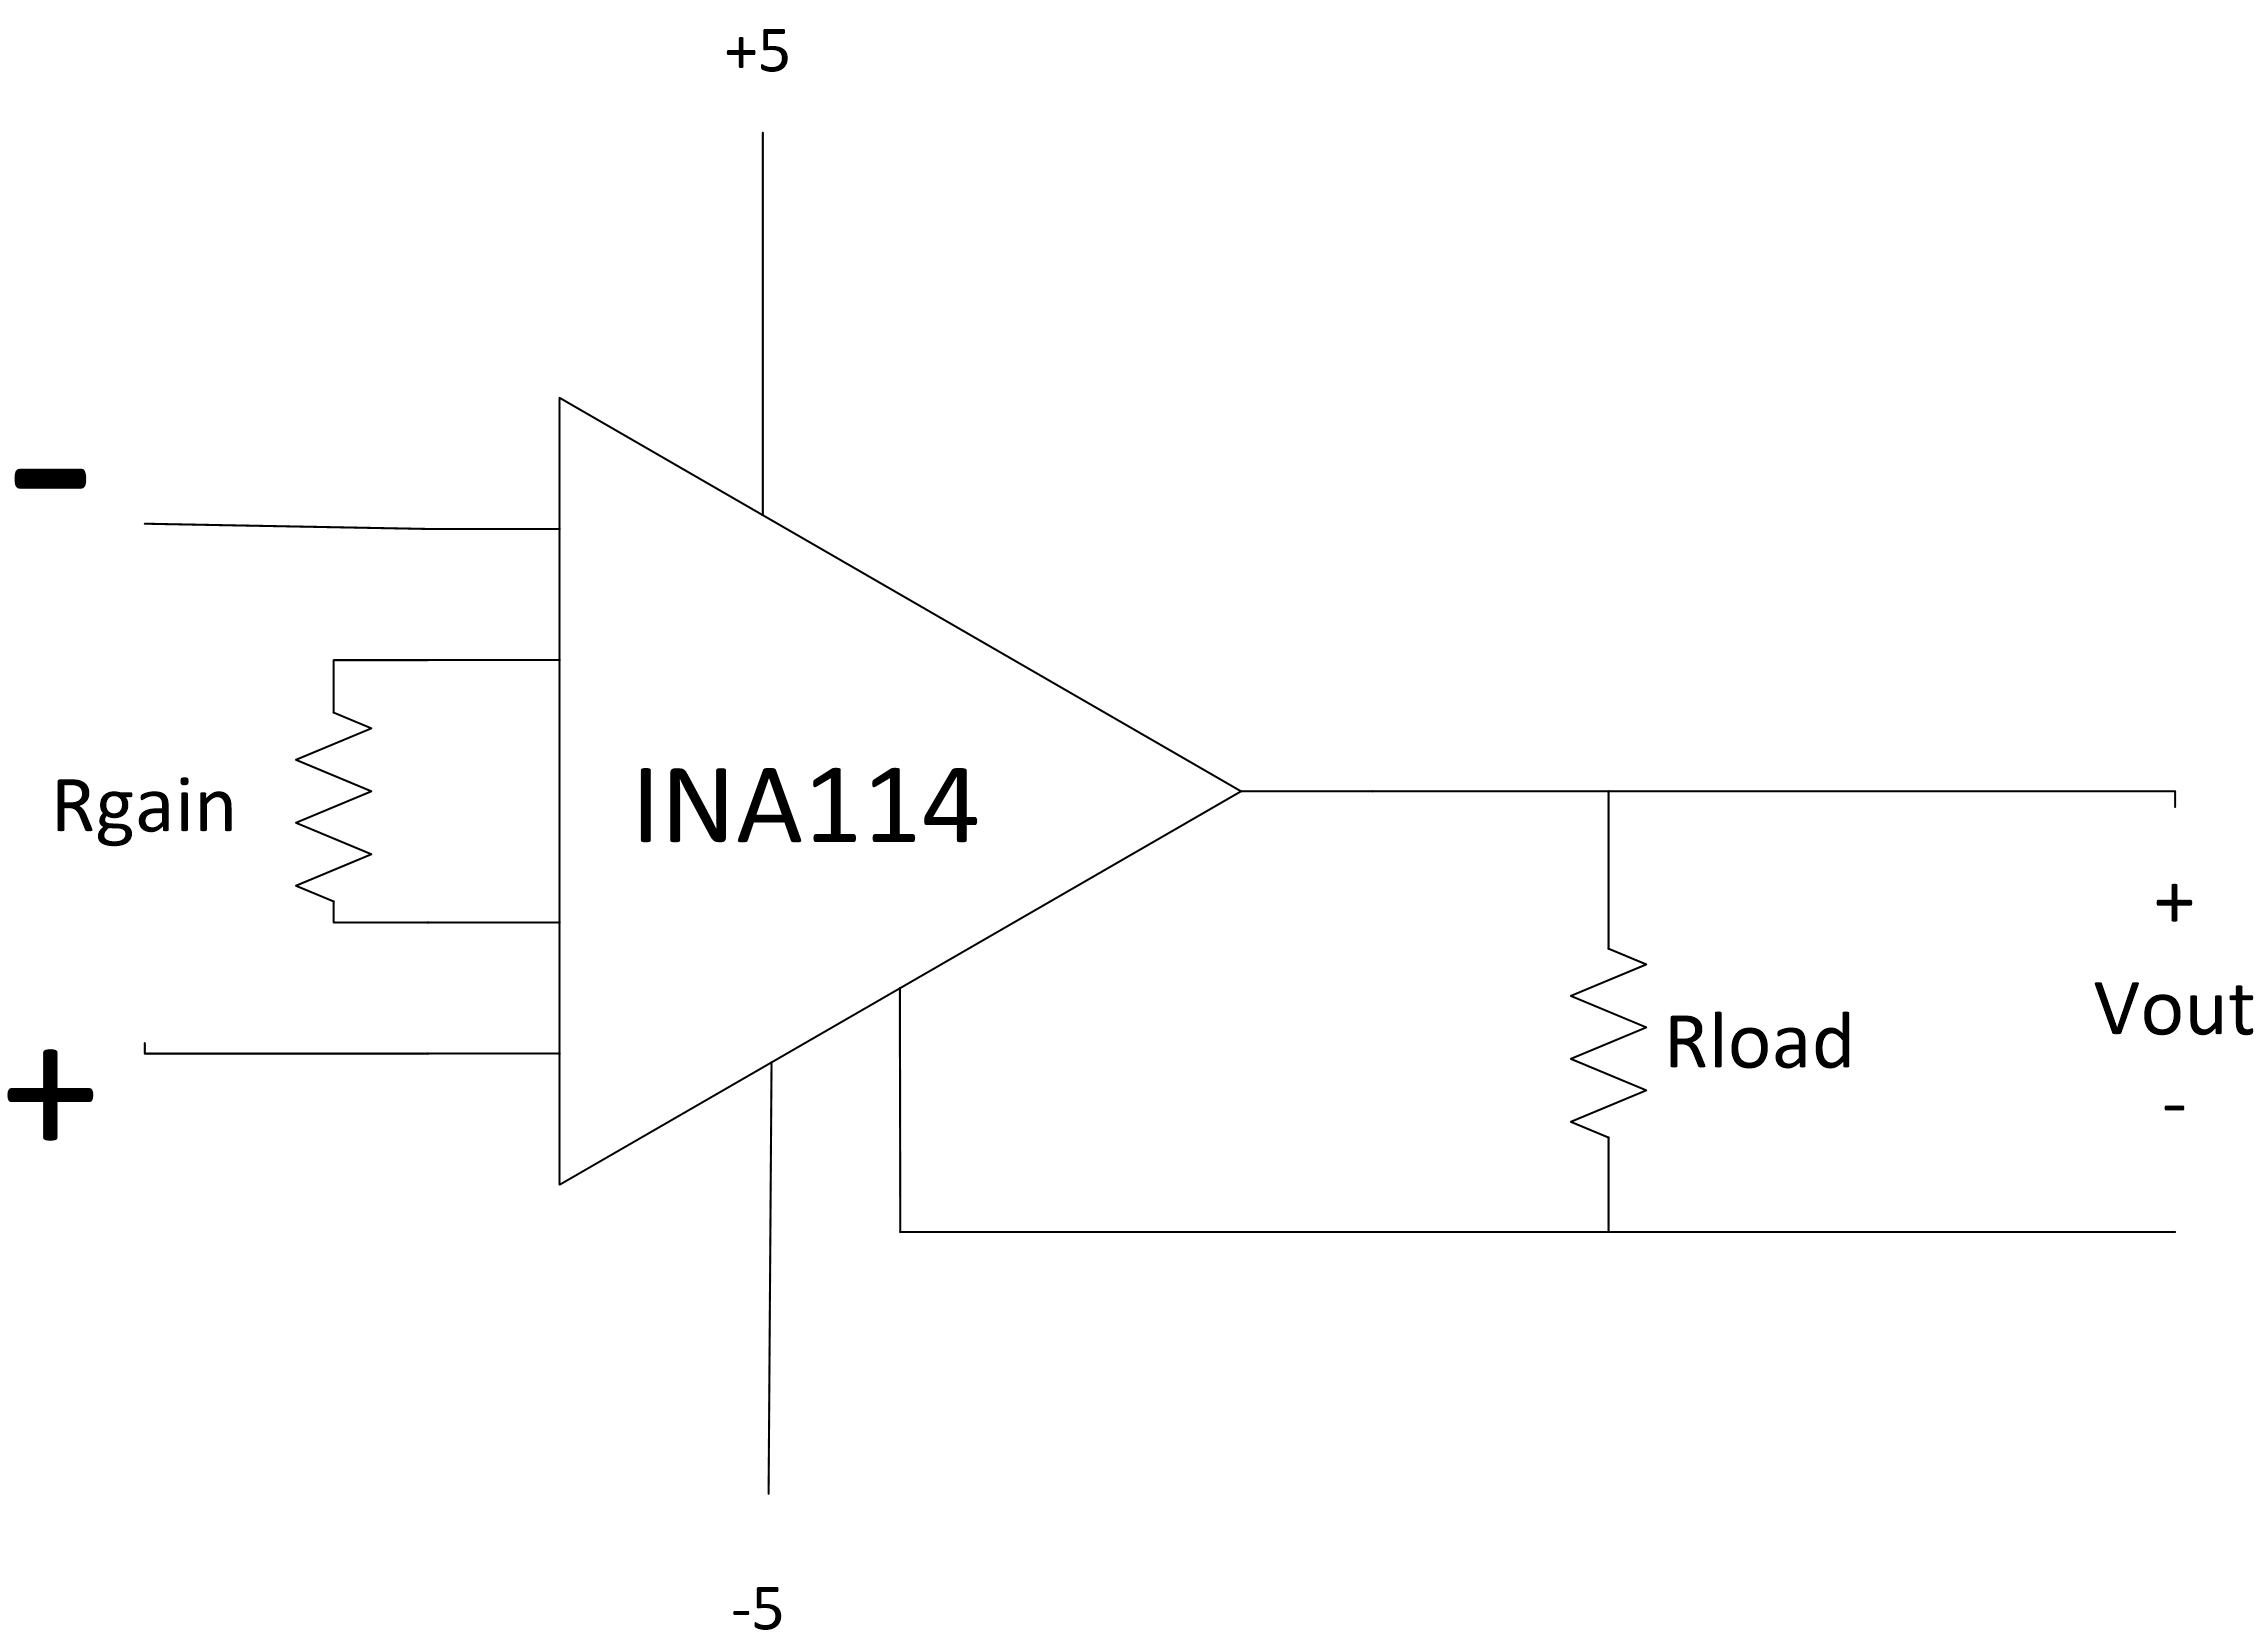
\includegraphics[width=0.6\textwidth]{Figurer/Hardware/Forstaerker}
	\caption{Der overordnede design af forstærkeren.}\label{labelpic}
\end{figure}



$R_{gain}$ er modstanden, som bestemmer, hvor meget forstærkning, instrumentationsforstærkeren skal give og $R_{load}$ er den belastning, der kommer efter kredsløbet. I dette tilfælde, er det, det analoge filter. For at finde $R_{gain}$’s størrelse, kræver det, at der vides, hvor meget forstærkning der er brug for. Dette findes, ved at bestemme den maksimale spænding, som transduceren kan give, i en blodtrykssituation. Dette regnestykke kan ses realiseret i ligning \ref{ligning1}:

\begin{align}
	VT_{max}=T_{max}\cdot V_{max}\cdot HG_{max}=\frac{\mu V}{V/mmHG}\cdot 5V\cdot 250mmHg=6,25mV
	\label{ligning1}
\end{align}

Spændingen ønskes at skaleres op til DAQ’ens dynamikområde, som ligger omkring de 5V. Forstærkningsfaktoren udregnes ved simpel brøkregning, som ses på ligning \ref{ligning2}:

\begin{center}
	\begin{align}
		G=\frac{5}{6,25 \cdot 10^{-3}}=800
		\label{ligning2}
	\end{align}
\end{center}

INA114’s datasheet giver en ligning for udregning af forstærkning. Da forstærkningen er kendt, omskrives ligning \ref{ligning3} , så modstanden $R_{gain}$’s værdi i stedet bestemmes:\\


\begin{align}
	Gain=1+\frac{50k\Omega}{R_{gain}}\to G-1=\frac{50k\Omega}{R_{gain}}\to \frac{50kOhm}{G-1}=R_{gain}
	\label{ligning3}
\end{align}

Herefter kan den ohmske værdi af $R_{gain}$ bestemmes, hvilket sker i linging \ref{ligning4}:

\begin{align}
	R_{gain}=\frac{50k\Omega}{800-1}=62,578 \Omega
	\label{ligning4}
\end{align}

\subsection{Design af analogfilter}
Filteret, som ses på figur \ref{fig:Filter}, skulle realiseres som et aktivt 2. ordens lavpasfilter med båndbredde på 50 Hz af typen Sallen-Key med unity gain (se \ref{fig:Filter}). Filteret skulle designes som et Butterworth filter med cut off frekvens på 50 Hz. C2 skulle vælges til 680 nF og R1 = R2. Operationsforstærkeren skal være af typen OP27.  

\begin{figure}[H]
	\centering
	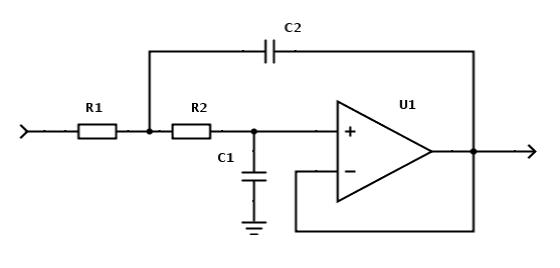
\includegraphics[width=1\textwidth]{Figurer/Hardware/FilterDesign}
	\caption{Unity gain 2. ordens Sallen-Key lavpas konfiguration}
	\label{fig:Filter}
\end{figure}

Der blev valgt en dæmpningsfaktor på 1, da det ville være mest optimalt med et kritisk dæmpet signal. Ud fra hjemmesiden\footnote{http://sim.okawa-denshi.jp/en/OPseikiLowkeisan.htm} fandt vi overføringsfunktionen for Sallen-Kay lavpasfiltret, udtrykt i ligning \ref{ligning5}:


\begin{align}
	\frac{V_{out}(S)}{V_{in}(S)}=\frac{\frac{1}{R_1C_1R_2C_2}}{s^2+s(\frac{1}{R_2C_2}+\frac{1}{R_1C_2})}+\frac{1}{R_1C_1R_2C_2}
	\label{ligning5}
\end{align}

Da det er blevet opgivet at $R1=R2$, kan overføringsfunktionen forkortes: 

\begin{figure}[H]
	\centering
	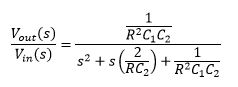
\includegraphics[width=0.35\textwidth]{Figurer/Hardware/ligning2}
\end{figure}

Dernæst sammenlignes med standardformlen for overføringsfunktionen for et andet ordens filter.

\begin{figure}[H]
	\centering
	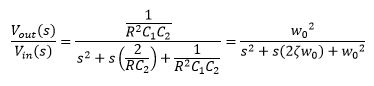
\includegraphics[width=0.6\textwidth]{Figurer/Hardware/ligning3}
	\label{fig:lign3}
\end{figure}

Ud fra dette kan regnes komponentværdierne for R, idet

\begin{figure}[H]
	\centering
	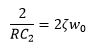
\includegraphics[width=0.2\textwidth]{Figurer/Hardware/ligning4}
	\label{fig:lign4}
\end{figure}

Ved hjælp af mathcad isoleres R.

\begin{figure}[H]
	\centering
	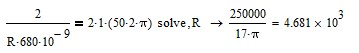
\includegraphics[width=0.85\textwidth]{Figurer/Hardware/ligning5}
	\label{fig:lign5}
\end{figure}

Dernæst kan komponentværdien for C1 udregnes, idet:

\begin{figure}[H]
	\centering
	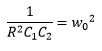
\includegraphics[width=0.2\textwidth]{Figurer/Hardware/ligning6}
	\label{fig:lign6}
\end{figure}

Ved hjælp af mathcad isoleres C1. 

\begin{figure}[H]
	\centering
	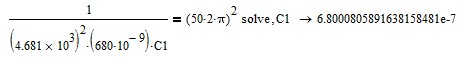
\includegraphics[width=0.9\textwidth]{Figurer/Hardware/ligning7}
	\label{fig:lign7}
\end{figure}

Derved er komponentværdierne for kredsløbet fundet og de ses indskrevet på \ref{fig:Filter}. 

\begin{figure}[H]
	\centering
	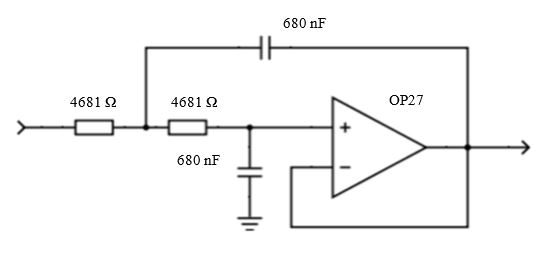
\includegraphics[width=1\textwidth]{Figurer/Hardware/FilterDesignMedKomponentvaerdier}
	\caption{Unity gain 2. ordens Sallen-Key lavpas konfiguration med indsatte komponentværdier.}
	\label{fig:Filter_K}
\end{figure}

Generelt er et unity gain Sallen-Key filter med equivalente capacitorer og equivalente resistore kritisk dæmpet dvs. en kvalitets faktor på 1/2. Dette kan også ses når komponentværdierne indsættes i ”Sallen-Key Low-pass Filter Design Tool”\footnote{http://sim.okawa-denshi.jp/en/OPseikiLowkeisan.htm}. Desuden ses bodeplottet nedenfor:

\begin{figure}[H]
	\centering
	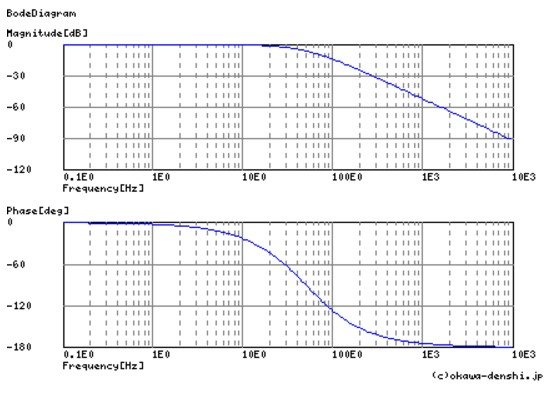
\includegraphics[width=1\textwidth]{Figurer/Hardware/Bodeplot}
	\caption[]{Bodeplot af overføringsfunktionen\footnotemark}
	\label{fig:Bodeplot}
\end{figure}
\footnotetext{http://sim.okawa-denshi.jp/en/OPseikiLowkeisan.htm}


\subsection{Grænseflader}

\section{Software arkitektur}
\subsection{GUI}
Dette afsnit beskriver hvilke tanker og overvejelser der er gjort i forbindelse med designet af diverse brugergrænseflader. Nedenfor ses udkast til disse brugergrænseflader.\\
Til designet af brugergrænsefladen er blevet udført ud fra de 16 principper for gode brugergrænseflader. Der er ligeledes i form1 hentet inspiration fra allerede eksisterende blodtryk monitor. I designet af brugergrænsefladen bestræbes, der efter at gøre det så virkelighedsnært som muligt ud fra de redskaber og oplysninger der er til rådighed.\\ \\
Brugergrænsefladen er inddelt i 3 forskellige interfaces. De 3 interfaces er henholdvis Log ind, Form1 og Gem. De personer, der interagerer med brugergrænsefladen er sundhedsfagligt personale som typisk vil være en læge eller sygeplejerske. Dette er der også taget højde for i designet da, der aldrig vil være andre end det sundhedsfaglige personale der interagerer med brugergrænsefladen og derfor er den en skærpet målgruppe.\\
Nedenfor kommer der en uddybende beskrivelse af brugergrænsefladen. 

\begin{figure}[H]
	\centering
	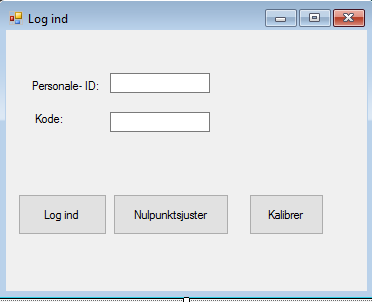
\includegraphics[width=0.7\textwidth]{Figurer/GUI/Logind_GUI}
	\caption{Login vindue}
	\label{Login vindue}
\end{figure}

I figur \ref{Login vindue} er der tage udgangspunkt i, at brugergrænsefalden skal være enkel og overskuelig opbygget. Der skal ikke være nogle overflødige ting og de knapper der er vigtige som bruger skal benytte skal stå tydeligt frem. Opbygningen skal afspejle brugerens logik.\\ \\ 
Tankerne omkring den enkle opbygning er, at hvis der opstår en akut situation hvor systemet skal i gang hurtigt skal det være nemt og hurtigt at logge ind i systemet. Det er vigtigt at knapperne er selvforklarende og giver brugeren det der forventes af knappen når den benyttes. \\ \\
Der er taget højde for feedback til bruger ved forkert log ind får brugeren en besked om at log ind er indtastet forkert og der skal prøves forfra. \\


\begin{figure}[H]
	\centering
	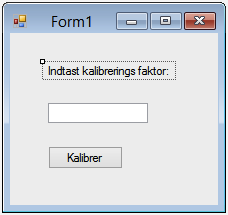
\includegraphics[width=0.7\textwidth]{Figurer/GUI/kalibrerGUI}
	\caption{Kalibrer vindue}
	\label{Kaliber vindue}
\end{figure}

Vist på figur \ref{Kaliber vindue}, hvor der her er lagt vægt på det funktionelle, med et enkelt og simpelt design. Der er vejledende tekst, som gør det nemt for aktøren at finde ud af systemet.

\begin{figure}[H]
	\centering
	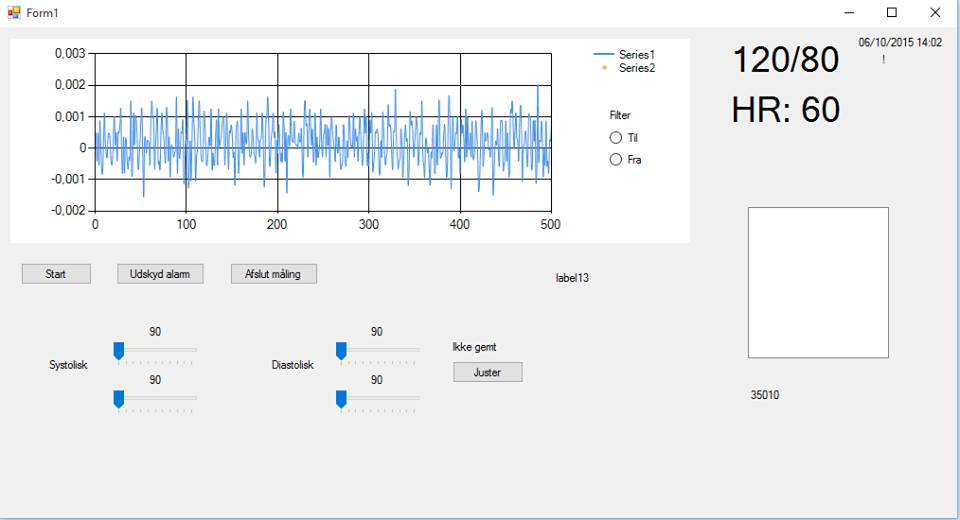
\includegraphics[width=1\textwidth]{Figurer/GUI/GUI_form1}
	\caption{Blodtryk vindue}
	\label{Blodtryk vindue}
\end{figure}

I blodtryksvinduet, vist på figur \ref{Blodtryk vindue}, er opbygningen mere kompliceret og med flere knapper end ved Log ind og Gem. Der er taget højde for at knapperne er selvforklarende og deres navne afspejler de bagvedliggende handlinger. Dette medfører at brugeren stadig har et overblik over brugergrænsefalden og stadig selv kan kontrollerer hvad der skal ske. Denne brugergrænseflade er ikke tiltænkt nye brugere, men derimod brugere der har et kendskab til den og til hvilke sundhedfaglige værdier og udtryk, der vises på den.  Derfor benyttes brugerens sprog på brugergrænsefalden og ikke et sprog med termer, der er forståelig for alle. 

\begin{figure}[H]
	\centering
	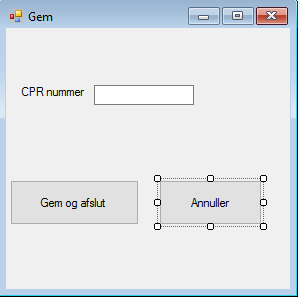
\includegraphics[width=0.7\textwidth]{Figurer/GUI/Gem_GUI}
	\caption{Gem vindue}
	\label{Gem vindue}
\end{figure}
\subsection{UML klassediagram}

På figur \ref{Gem vindue}, gemme-vinduet, er der igen taget udgangspunkt i en enkel opbygning og at knapperne, der skal bruges er tydelige og selvforklarende. Det er her også brugerens logik, der afspejles og ingen unødvendige ting er inddraget i brugergrænsefalden. Det er her muligt at afbryde situationen ved at der er en alternativ udvej, som kan bruges hvis den op startet handling fortrydes. Der er taget højde for feedback til brugeren hvis der indtastes forkert CPR nummer får brugeren det af vide i et pop-up vindue. 

\subsection{Appliktationsmodel}

\subsubsection{Klassediagram}

\subsubsection{Domænemodel}
Diagrammet viser en domæne model for blodtryks systemet. Dette diagram giver et godt overblik over systemet som helhed og hvilke elementer, der indgår i systemet. Diagrammet viser hvordan brugeren interagerer med systemet og hvordan systemet forløber efter det igangsættes af bruger. 

\begin{figure}[H]
	\centering
	\includegraphics[width=1\textwidth]{Figurer/ISE/Domaenemodel}
	\caption{Domænemodel}
	\label{domaenemodel}
\end{figure}

\subsubsection{Sekvensdiagram}
Sekvensdiagrammet er et interaktions diagram, der viser hvordan processer i systemet forløber. Use casene ligger til baggrund for udarbejdelsen af sekvensdiagrammerne.\\ \\
Der er blevet lavet et sekvensdiagram for hver use case for at give det bedste overblik over hver handling i forhold til systemet. I sekvensdiagrammet har vi brugt virtuelle metode kald til at beskrive forløbet. I use case 2-7 er det brugeren, der interagerer med systemet og er initiator for a handlingerne bliver udført.

\begin{figure}[H]
	\centering
	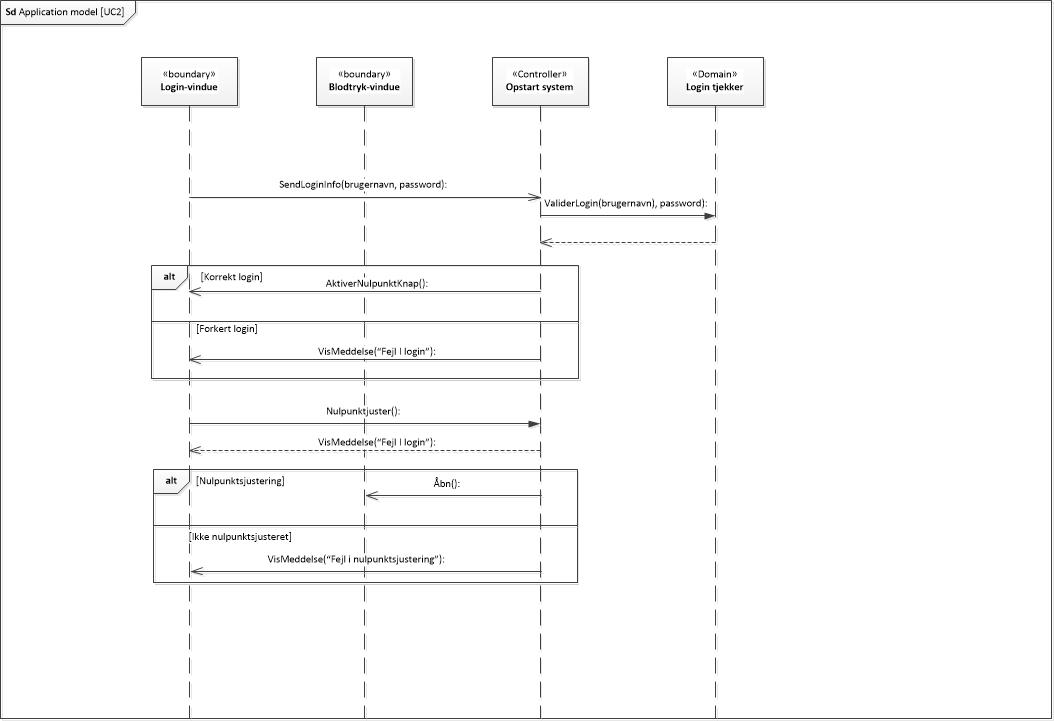
\includegraphics[width=1\textwidth]{Figurer/ISE/sdAppModelUC2}
	\caption{Sekvensdiagram UC2}
	\label{sd UC2}
\end{figure}

På figur \ref{sd UC2} ses det hvordan brugeren logger ind i systemet og hvordan brugeren for systemet nulpunktsjusteret. Det er brugeren, der interagerer med systemet og er initiator for at handlingerne bliver udført. 

\begin{figure}[H]
	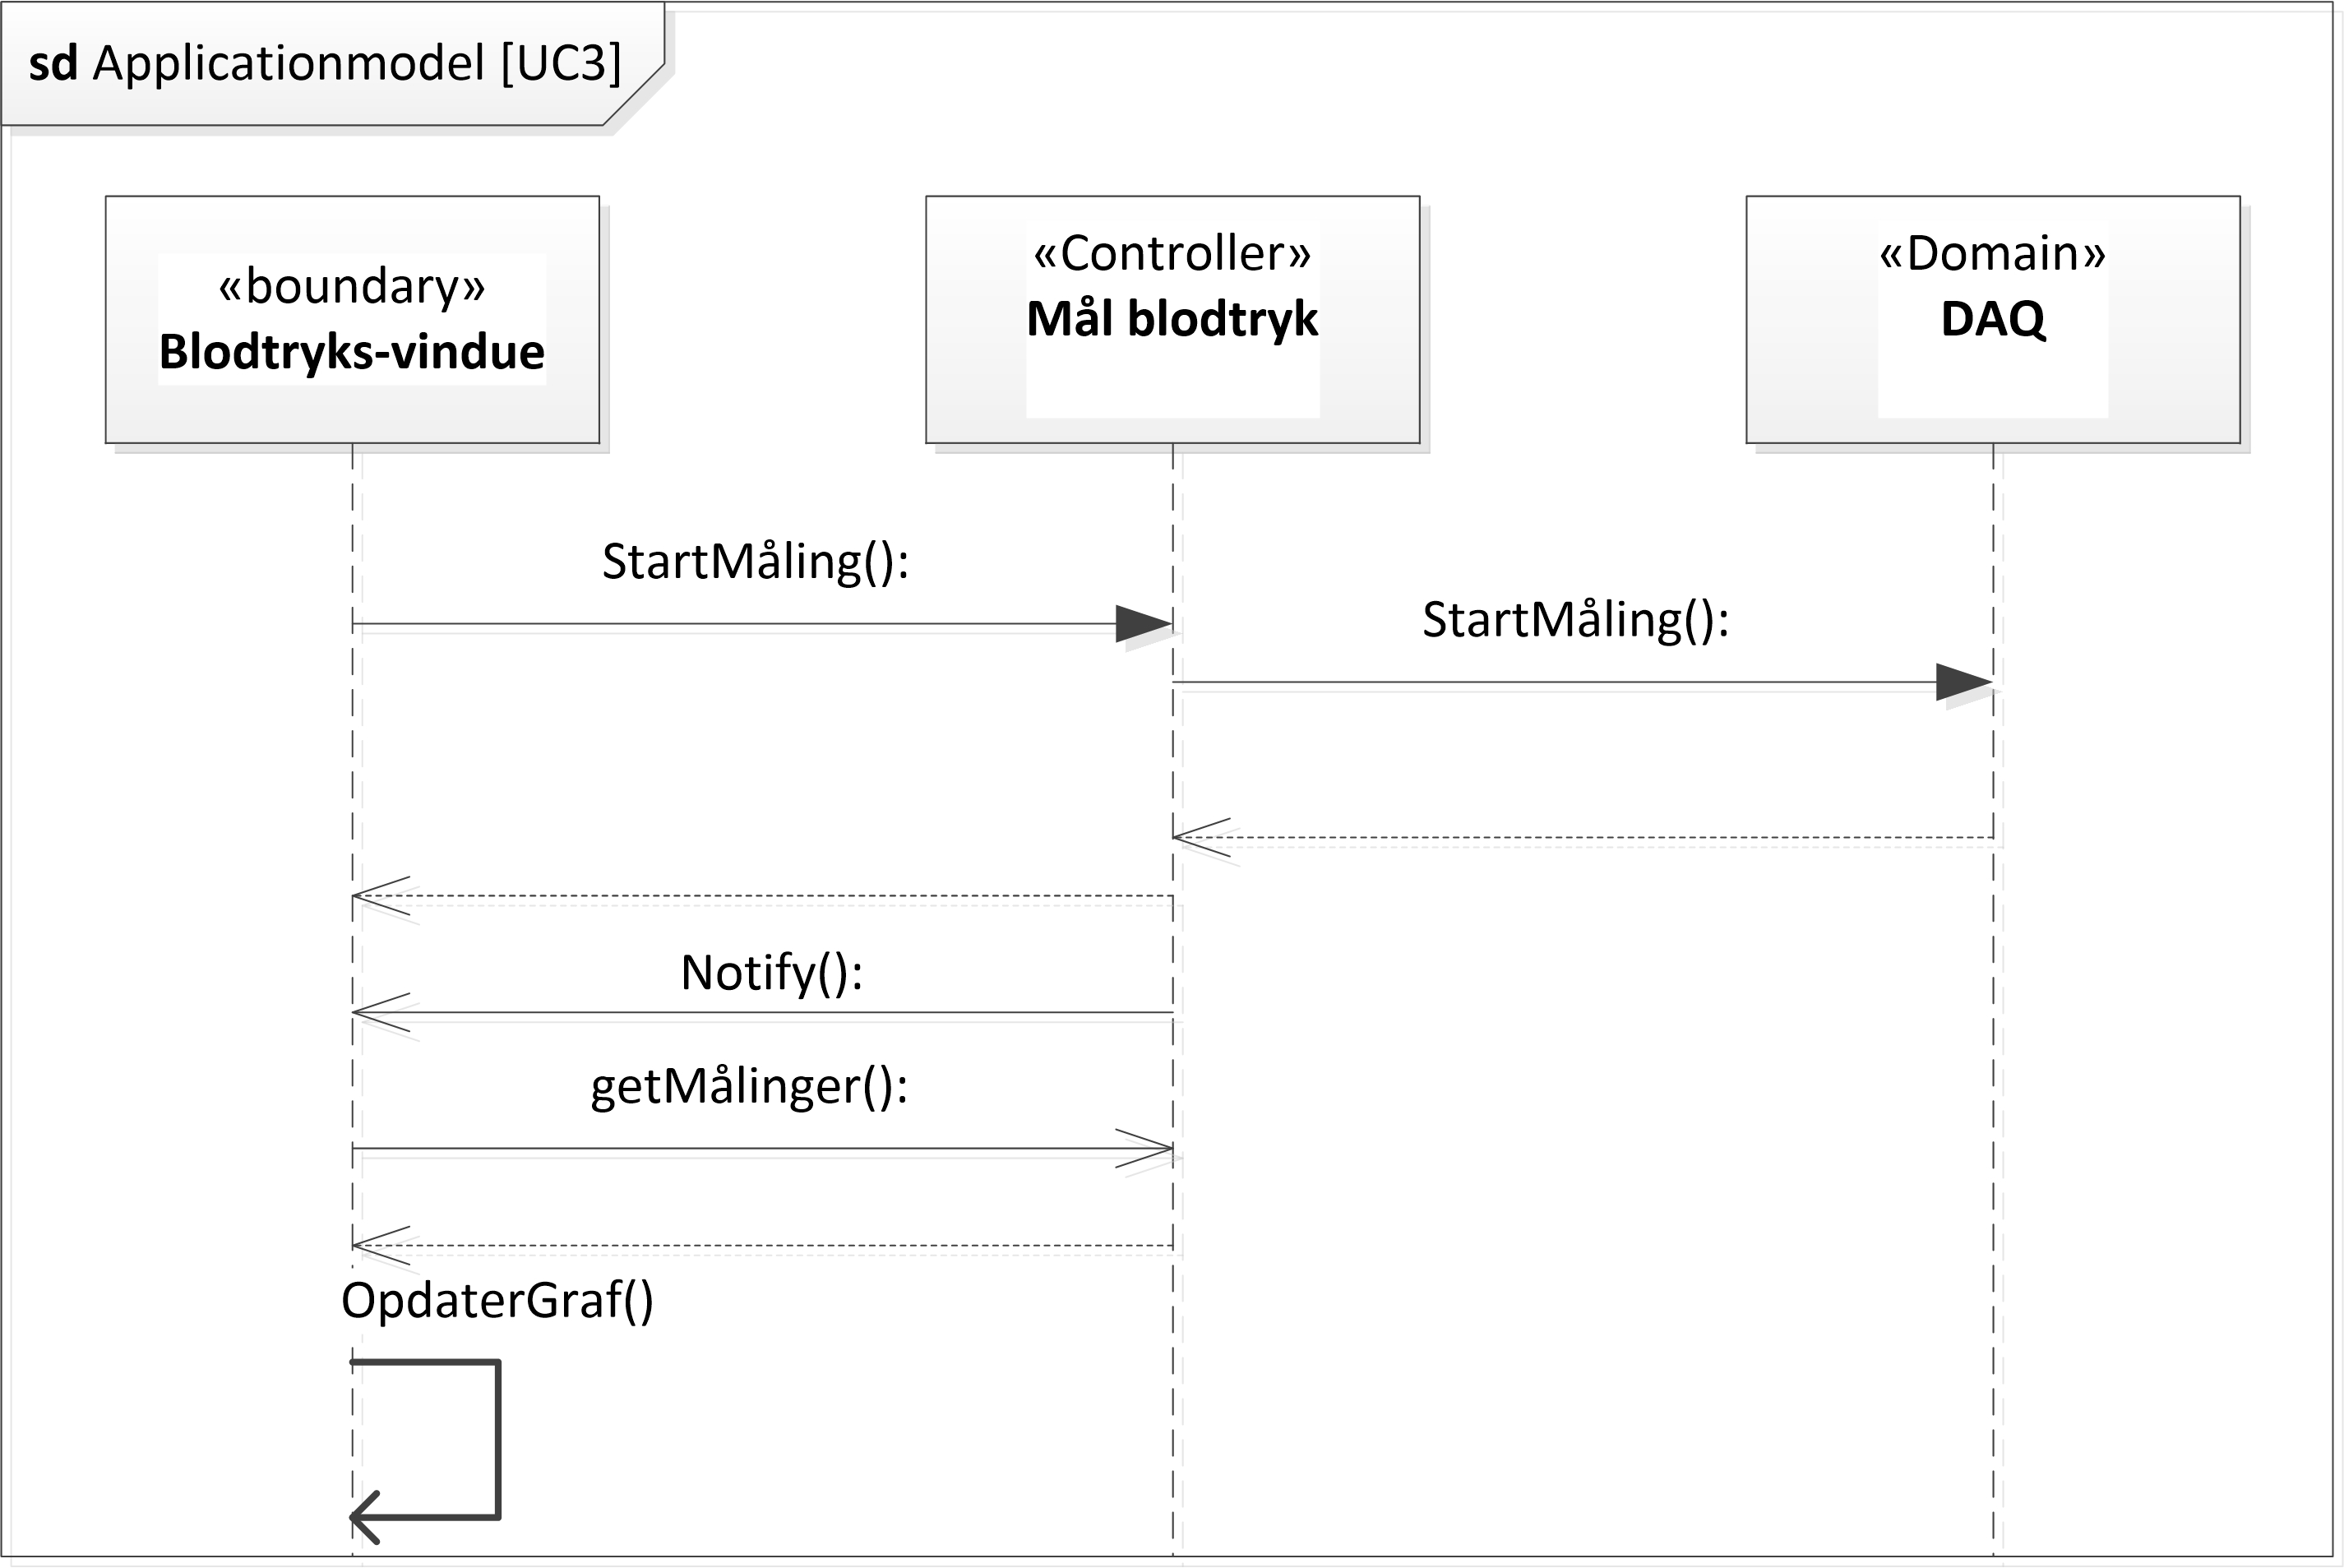
\includegraphics[width=1\textwidth]{Figurer/ISE/sdAppModelUC3}
	\caption{Sekvensdiagram UC3}
	\label{sd UC3}
\end{figure}

Figur \ref{sd UC3} viser hvordan brugeren starter målingen og hvordan graferne vises på brugergrænsefalden.

\begin{figure}[H]
	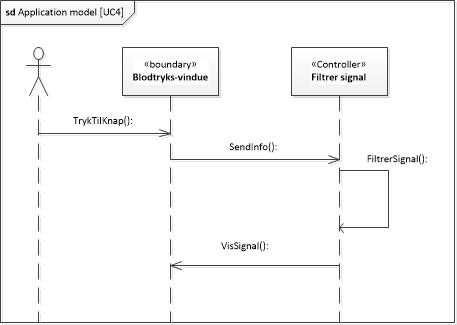
\includegraphics[width=1\textwidth]{Figurer/ISE/sdAppModelUC4}
	\caption{Sekvensdiagram UC4}
	\label{sd UC4}
\end{figure}

I sekvensdiagrammet figur \ref{sd UC4} ses hvordan brugeren kan vælge om blodtrykssignalet skal filtreres eller ej.

\begin{figure}[H]
	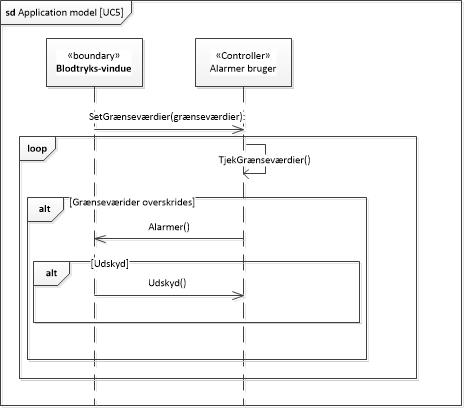
\includegraphics[width=1\textwidth]{Figurer/ISE/sdAppModelUC5}
	\caption{Sekvensdiagram UC5}
	\label{sd UC5}
\end{figure}

Det ses på figur \ref{sd UC5} hvordan brugeren justerer grænseværdierne for patientens blodtryk. Denne justering sker ud fra patientens målte blodtryk. De justerede grænseværdi ligger til grundlag for alarmen. Desuden viser figuren, at brugeren har mulighed for at udskyde alarmen.

\begin{figure}[H]
	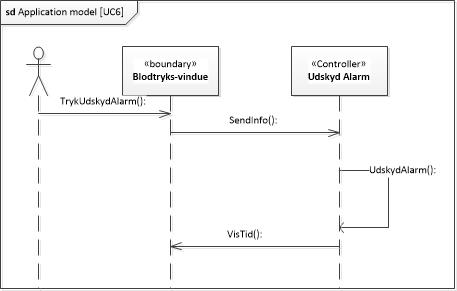
\includegraphics[width=1\textwidth]{Figurer/ISE/sdAppModelUC6}
	\caption{Sekvensdiagram UC6}
	\label{sd UC6}
\end{figure}

Figur \ref{sd UC6} viser hvordan systemet gemmer og afslutter en måling. 

\subsubsection{Opdateret Klassediagram}
Klasse applikationsmodellerne er udarbejdet ud fra use casene, sekvensdiagrammer og domænemodellen. Der er ligesom ved sekvensdiagrammerne lavet et klassediagram for hver use case. Der er her også brugt virtuelle metoder. 

\begin{figure}[H]
	\centering
	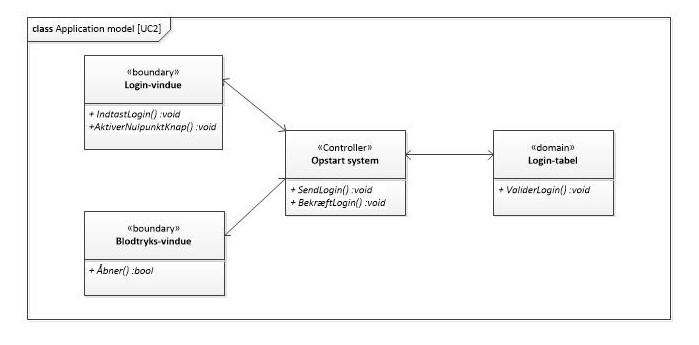
\includegraphics[width=1\textwidth]{Figurer/ISE/classAppModelUC2}
	\caption{Klassediagram UC 2}
	\label{classApp UC2}
\end{figure}

\begin{figure}[H]
	\centering
	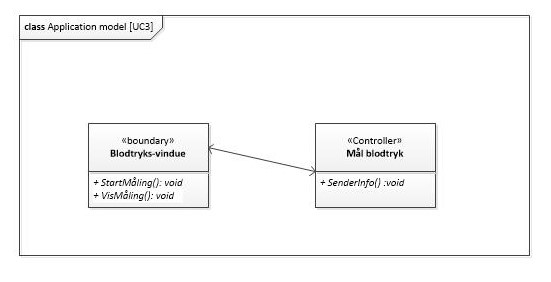
\includegraphics[width=1\textwidth]{Figurer/ISE/classAppModelUC3}
	\caption{Klassediagram UC 3}
	\label{classApp UC3}
\end{figure}

\begin{figure}[H]
	\centering
	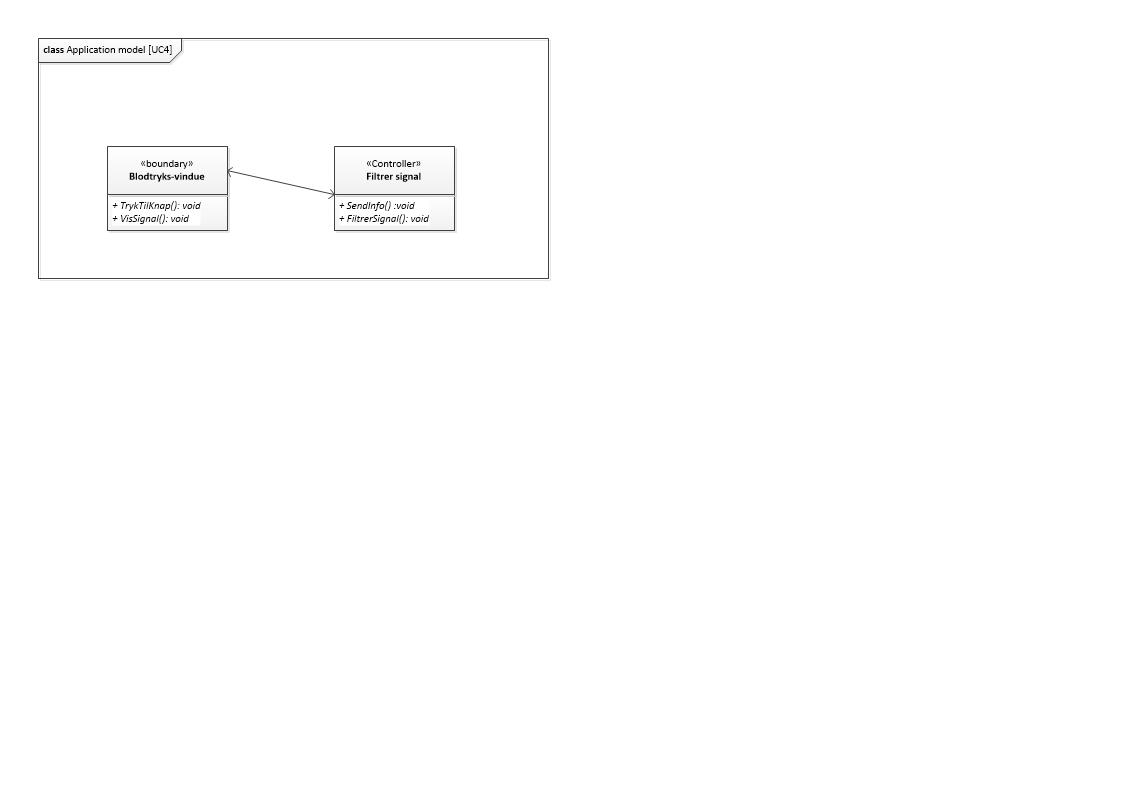
\includegraphics[width=1\textwidth]{Figurer/ISE/classAppModelUC4}
	\caption{Klassediagram UC 4}
	\label{classApp UC4}
\end{figure}

\begin{figure}[H]
	\centering
	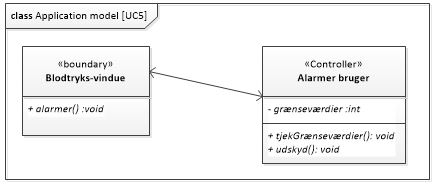
\includegraphics[width=1\textwidth]{Figurer/ISE/classAppModelUC5}
	\caption{Klassediagram UC 5}
	\label{classApp UC5}
\end{figure}



\begin{figure}[H]
	\centering
	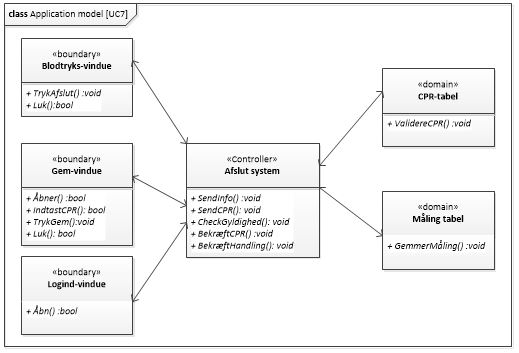
\includegraphics[width=1\textwidth]{Figurer/ISE/classAppModelUC7}
	\caption{Klassediagram UC 7}
	\label{classApp UC7}
\end{figure}

\section{Software implementering}



 







